\documentclass[12pt,twoside]{mitthesis}
\usepackage{lgrind}
%% These have been added at the request of the MIT Libraries, because
%% some PDF conversions mess up the ligatures.  -LB, 1/22/2014
\usepackage{cmap}
\newtheorem{theorem}{Theorem}
\renewcommand{\theenumii}{\theenumi.\arabic{enumii}}
\renewcommand{\labelenumii}{\theenumii}
\usepackage{graphicx}
\usepackage{enumerate}
\usepackage{enumitem}
\usepackage{color}
\usepackage[T1]{fontenc}
\pagestyle{plain}

%\usepackage{biblatex}
%\addbibresource{reference.bib}

\renewenvironment{abstract}{%
    \clearpage
    \null\vfil
    \begin{center}%
        {\bfseries \abstractname}%
    \end{center}%
    }
{\endquotation\vfil\null\clearpage}


\begin{document}


\begin{center}
\large\textbf{U Network: The Decentralized Content Valuation \& Publishing Platform}
\end{center}
\vspace{1cm}


\begin{center}
\large\textbf{Technical White Paper}
\end{center}

\begin{center}
\textbf{version 0.2.0}

\end{center}
\vspace{4cm}

\begin{center}
\textit{Draft for open community review and subject to change.}
\end{center}

\pagestyle{empty}


%  abstract
\renewcommand{\abstractname}{\bf \Large Abstract}
\begin{abstract}

\emph{U Network}\footnote{\emph{U Network}: http://www.u.network} is the revolutionary content-value based prediction market platform and a content-incentive ecosystem driven by value. \emph{U Community} is the first digital asset platform powered by \emph{U Network}.

\emph{U Network} leverages the blockchain technology to build a prediction market of user-generated content. By constructing a more effective pricing system for the generated content, users are motivated to discover and promote high-value contents by sharing it with other participants in the network. In particular, \emph{U Community} is built on top of \emph{U Network}, which consist of four types of participants: content creators, content explorer, community moderators and regular user. All these participants interact with each other and build the community. With the help of prediction market, content creators and explorers are encouraged to keep generating and discovering high-quality contents in \emph{U Community}, therefore, offering plenty of value to regular users. Community moderators are periodically selected from regular users and entitled with important privilege(e.g., deleting improper contents) to maintain the normal operation of community. Moreover, a voting-based appeal mechanism is built to prevent abusing their privilege. As monetized incentive, regular users need to pay tokens of \emph{U Network} to access valuable contents, while content creators, explorers and moderators will be rewarded with tokens for their services.

The goal of \emph{U Network} is to build a decentralized user-generated-content blockchain platform where users are encouraged to create and explore valuable contents with monetized incentive. \emph{U Community} will be the first application built on this platform with high-accessibility, high-scalability, and low latency.


\vspace{1cm}

\textbf{Keywords:} Digital Asset, Prediction Market, Blockchain, Monetized Incentive
\end{abstract}

% list of contents - automatically generated, do not change
\pagestyle{plain}
  % -*- Mode:TeX -*-
%% This file simply contains the commands that actually generate the table of
%% contents and lists of figures and tables.  You can omit any or all of
%% these files by simply taking out the appropriate command.  For more
%% information on these files, see appendix C.3.3 of the LaTeX manual. 
\tableofcontents
%\newpage
%\listoffigures
%\newpage
%\listoftables



% chapter 1: introduction
\chapter{Introduction}
\section{Background}
%%% discuss huge volume of contents and why content valuation is needed 
\subsection{Inforamtion Overload}
In the age of information explosion, people are overwhelmed by the redundant content and data. As shown in the figure \ref{fig:data}, volume of data has experienced exponential growth recently and this trend will continue in the next few years.

\vspace{5pt}
\begin{figure}
\centering
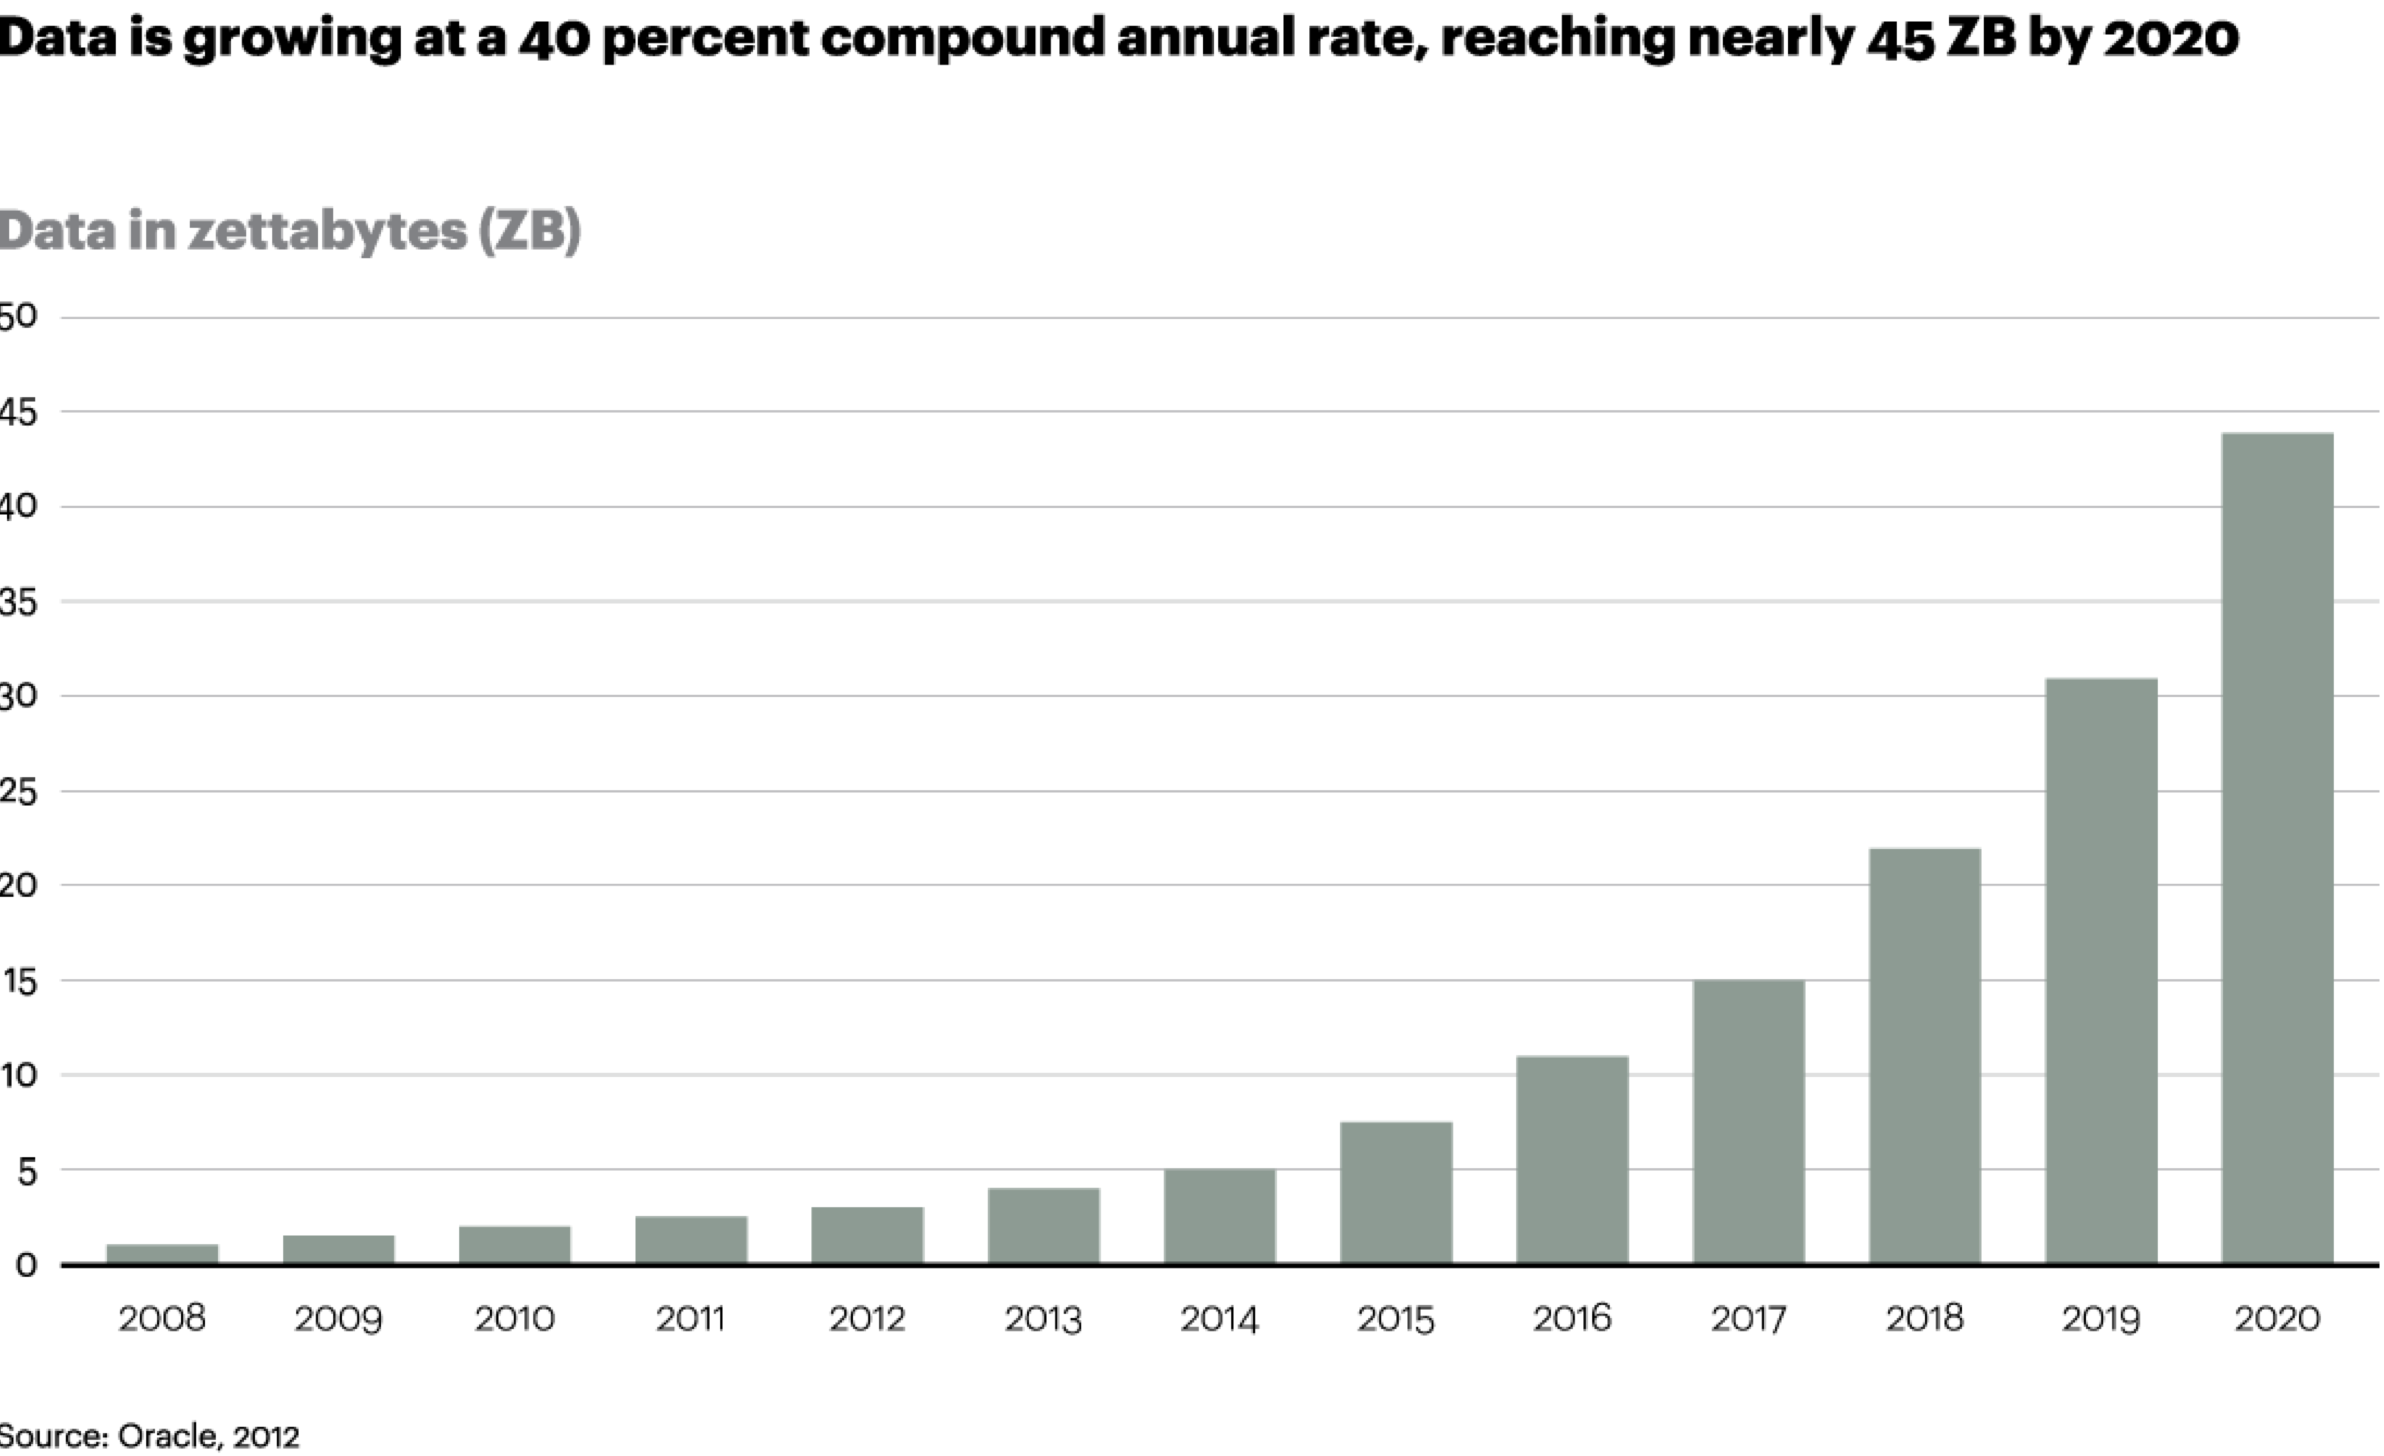
\includegraphics[width=\linewidth]{data_grow.png}
\caption{Exponential Growth of Data Information}
\label{fig:data}
\end{figure}

%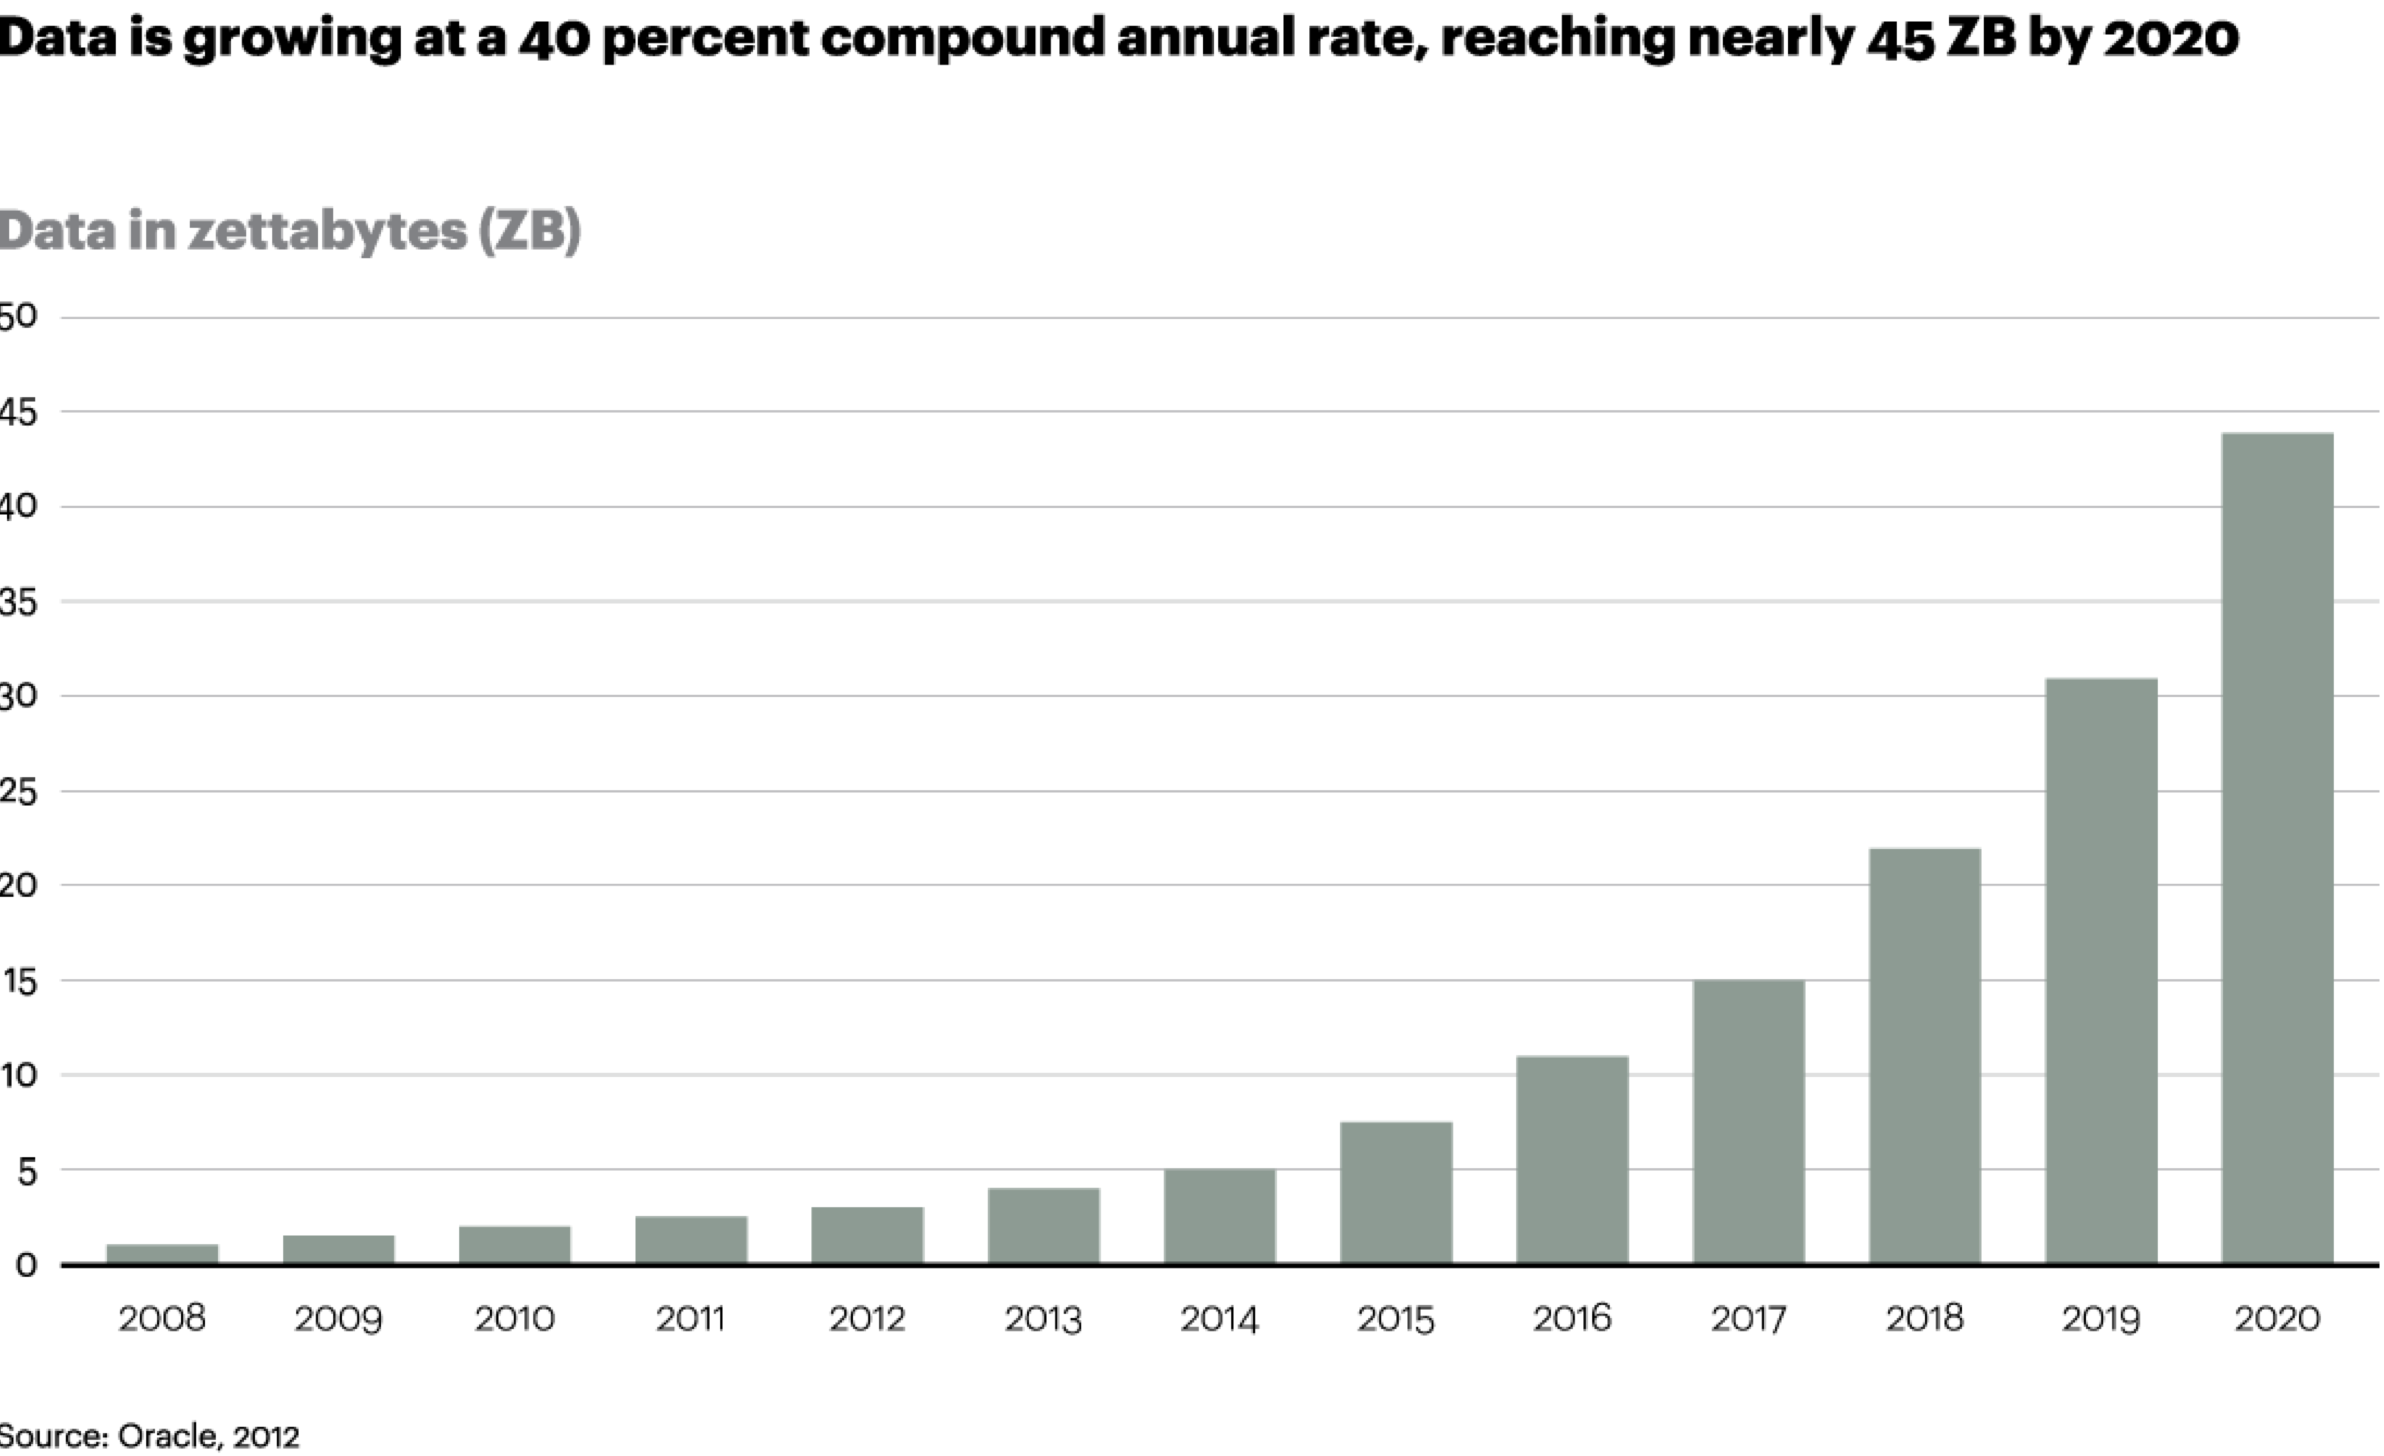
\includegraphics[width=\linewidth]{data_grow.png}

With the rapid growth of Internet, more information are generated and shared across the world with ever-faster speed, which causes several issues:
\begin{itemize}
\item \textbf{Low Quality Issue}: Many content creators generate large volume of contents without paying attention to quality, therefore, adding more superficial, distracting, or eye-catching contents with low quality. As such, audience can easily ignore high-value contents due to the interference of low-quality contents. 
\item \textbf{Copyright Issue}: Several content creators simply copy others' contents from the Internet and publish to their audience with/without modification, which is actually plagiarism and infringement. In current environment, it is really hard to trace back the original copyright ownership of one piece of content. 

\end{itemize}
Therefore, it becomes urgent but extremely challenging to identify those high-value contents from vast amount of information and reward original owners with less effort. 

\subsection{Problems of Centralized Platforms}
Existing user-generated-content communities, such as Facebook, Youtube, Wikipedia and Twitter, usually have their own centralized authorities, which monitor and control the operation of the entire community. They have several drawbacks as following:

\begin{itemize}
\item \textbf{Biased Content Judgment}: those authorities have all privileges, such as promoting, recommending, and deleting contents. In this scenario, only those authorities have the rights to promote high-value contents, so they may generate biased judgment according to their own criteria. The regular audience in those communities have no opportunity to promote their valued contents.

\item \textbf{Centralized Content Storage}: In those communities all user-generated-contents are stored in the centralized server or data center, which may cause service interrupt or outage when the centralized storage fails.  Much worse, the contents may be damaged or even lost and no longer available to be accessed. 

\item \textbf{Unfair Distribution of Benefits}: Usually the communities takes most income distribution from advertisement or audience payment, while content creators receive a very small piece or even no benefit at all.  

\end{itemize}
Those drawbacks make existing communities less attractive to contents creators and audience, because they are note motivated to create and promote high-value contents. 


\section{Why \emph{U Network} ?}
The solution to those issues of existing user-generated-content platforms is \emph{U Network}, which has following functionality:
\begin{enumerate}
    
    \item \textbf{discovering high-quality content}: By leveraging a decentralized prediction market to assess the quality of a content, \emph{U Network} provides an efficient way to find out high-quality information and avoids prejudice.    
    \item \textbf{reasonably distributing benefit}:  \emph{U Network} allocates monetized token rewards to the platform contributors with the help of content pricing mechanism. The contributors includes both content creator and any regular users who promote valuable contents with up-votes.
    
    \item \textbf{decentralizing content storage}: \emph{U Network} will support IPFS protocol (InterPlanetary File System\cite{ipfs}), a persistent internet file transfer protocol, or Genaro Network, a fault tolerant, tamper-resistant, permanent storage protocol. These decentralized storage solutions not only improve the reliability of data integrity but also guarantee the availability of contents using redundant copies across distributed server nodes.       
\end{enumerate}

\subsection{Mission of \emph{U Network}}
The mission of \emph{U Network} is to build a user-generated-contents community based on blockchain technology, which is a content-value based prediction market driven by quality and value of contents. This platform has following advantages compared with existing communities:
\begin{itemize}
\item content creators are motivated to generate more high-quality contents, because they receive monetized token rewards when their contents receive up-votes from more audience. 
\item all participants can receive token rewards when they promote high-value contents with up-vote. This is because contents with more up-votes will be assigned higher priority and become much easier to be accessed by audience.
\item Each up-vote in  \emph{U Network} costs certain amount of tokens, which is similar to \emph{Gas} in Ethereum network and represents the price of up-vote that users need to pay. This cost of up-vote becomes the income source of token rewards that distributed to contributors, and prevents malicious users gaming the up-vote mechanism for rewards. 
\end{itemize}

As such, more valuable contents will be generated in this community and all participants are motivated to discover and promote those high-value contents. 

From the theoretical point view, this motivation model is derived from ``efficient-market hypothesis'' \cite{efficient}.  The efficient-market was first introduced by Bachelier, who first recognized the efficiency of the market in selecting information. In short, the discounting of past, present, and future events have their reflections in the current market price. His theory assumes that investors in the market are rational and are looking for their self interest in maximizing their own profits, and each individual has an independent analysis of the value of a content. Therefore, it becomes feasible to leverage the wisdom of all participants in this community to set a price for each content, where the price serves as an accurate prediction of the true value.  

\subsection{Content-Value based Prediction Market}
The key component of  \emph{U Network} and affiliated communities is the prediction market. In principle, prediction market\cite{prediction} is a platform where people trades the outcome of events. In this prediction market, people receive profit if their predictions proved to be correct. The reward distribution follows a simple but fair and robust principle: reward is transferred from inaccurate predictors to accurate ones. Knowing this rule, people would try their best effort to gather more information and make their best predictions to receive the rewards.

The construction of the  \emph{U Network} prediction market follows the similar idea. Users can up vote to promote a piece of content with the cost of some \emph{U Network} tokens. If other audience think the current prediction underestimate the value of contents, they may up vote with more tokens. In this way, the cost of up-vote for high-quality contents keeps increasing, and accordingly the user who promote this content with up-vote can gain monetized token reward. 

To sum up,  \emph{U Network} will be constructed to be a content-value driven platform powered by blockchain. It is revolutionary to use the content-value prediction market to motivate all participants to discover and promote high-quality contents using token incentives. Therefore, it becomes much easier to discover high-quality contents with great value in the user-generated-content community.








% chapter 2: U network Design
\chapter{\emph{U Network} Platform Design}
\section{Design Principle}
\emph{U Network} follows two simple but critical principles in building an efficient content-value prediction market.
\begin{theorem}
There Ain't No Such Thing As A Free Lunch
\end{theorem}
In an efficient market, there ain't no such thing as a free lunch\footnote{tanstaafl: https://www.investopedia.com/terms/t/tanstaafl.asp}. One has to pay certain cost or price in order to gain profit. In \emph{U Network}, any user needs to pay certain amount of \emph{U Network} tokens to up-vote a piece of contents, and receive token rewards if the content prove to be high-quality with more value eventually. 

Following this policy, any expected profit reward has to cost an initial price payment. The other advantage of this principle is to prevent malicious users gaming or cheating this market mechanism for profit.

\begin{theorem}
 Principle of Fairness
\end{theorem}
To build an efficient market, it is imperative to treat every participant to be equal. First of all, every participant in the market should be able to receive incentive rewards that are proportional to his/her contribution. It is similar to stock options in startup companies where major contributors receive more stock rewards than others due to their significant contributions. 

In addition, every ``contribution'' should be appreciated and valued equally. Any one who contribute time and effort to create, discover, and distribution high-value contents should be valued equally and receive rewards. Towards this end, when users pay tokens to up-vote the contents, \emph{U Network} assigns portion of tokens to creators for rewarding their contribution, which further inspire them adding more high-quality contents. In the same time, users who promote these contents using tokens in their up-votes can also receive rewards for successfully discovering valuable contents. 

As such, the \emph{U Network} platform implements a mechanism that redistributes token income to both creators and up-voters.  Moreover, users who discover valuable contents early receive higher expected rewards than those late. This mechanism encourages users to early discover high-quality contents, therefore, making valuable contents easier to stand out. 

\section{Economic Incentive Design}
To create an efficient content-value driven prediction market, the most important component is the incentive mechanism. In this section, we further explain the economic incentive design in \emph{U Network}.

\subsection{Cost of Voting}
In \emph{U Network} , any up-vote would cost a small amount of tokens, but how to determine the amount of tokens for each vote (denoted as $C$)? 

//TODO each upvote should be a fixed cost, but token is with a floating price  

\subsection{Author Reward}
According to the sequential order of upvoting, the cost of \emph{U Network} tokens coming from all up-voters will be distributed to the creator and early up-voters. The formula of author reward is derived from harmonic series: 
\begin{center}
$$R = \sum_{k=1}^{N}  C_{k} * 1/{k}$$
\end{center}
$N$ is the total number of upvotes within a given period of time. $k$ is the rank of each up-vote. $C_{k}$ is the cost for $k$-th up-vote. 

In this case, all of the token payment from the \emph{first} up-voter would be distributed to the author, while only half of the token payment from the \emph{second} up-voter will be paid to the author. 

Another part of author reward comes from author reward pool.
//TODO our details of distributing rewards.

\subsection{Content Explorer Reward}
The up-voters who explore and promote high-quality contents with tokens will receive rewards for their contributions to the community. The reward formula for explorer $R_r$ is below:
\begin{center}
$$R_r = C * \sum_{k=r+1}^{N} 1/{(k)}$$
\end{center}
$r$ is the rank of explorer or up-voters. If the total number of up-voters is fixed, the earlier up-votes receive higher expected rewards. This mechanism distributes more incentives to up-voters in the early stage, therefore, it encourages voters to discover valuable contents earlier.
 
According this formula, the second up-voter would only contribute $1/2$ tokens to the content author, while the remaining $1/2$ tokens would be paid to the \emph{first} up-voter. As such, the third up-voter would pay $1/3$ token to each of content author, first up-voter, and the second up-voter. It's mathematically provable that the first $35\%$ of up-voters have positive expected return.     
\begin{center}
$$R_r = C * \sum_{k=r+1}^{N} \frac{1}{k}$$ 
\end{center}
Simple arithmetic calculation proves that up-voter can expect positive expected return:
\begin{center}
$$R_r \geq C \texttt{ if and only if } {r}>=0.35*{N} $$
\end{center}
In this mechanism, the content author would take the largest piece of the income benefit. And early up-voters will have positive expected returns as an incentive reward for exploring quality content earlier. 


\subsection{Other Contributor Rewards}
At this point, there is a question that may rise: ``What if users do not have any \emph{U Network}  tokens? Can they still contribution to the community?''

The short answer is no,users without \emph{U Network}  token can still contribute time and attention instead of paying token for up-vote. Based on Principle No.1 (There Ain't No Such Thing As A Free Lunch), users can receive \emph{U Network}  points by spending time and energy in completing micro tasks for the community. For example, they may receive points by signing-in daily, referring friends and distributing the high-quality contents to other channels. These points can be converted into \emph{U Network}  tokens with fixed 1 : 1 ratio and thus used for voting.  

To prevent malicious spam sign-up and web-bot attack, we impose a restriction: there is a dynamic hard-cap on how many points one single user can earn considering the community economy and user activities. As such, users are encouraged to create or promote valuable contents to earn \emph{U Network} tokens without limit or cap. 

\subsection{Delayed Settlement}
After each content is created, there is a period of time window in which the topic is open to critique from community users. If the content is eye-catching but violates the community policy (i.e., violent and sexual contents), the rewards to the author may be revoked or contributed to the \emph{U Network} reward pool for public goods in the community. The length of the time-period is set to be 7-days but can be changed dynamically upon the agreement of the community users.

\subsection{Downvote}
Existing user-generated-content communities rarely have down-vote options. To fully distinguish valuable contents from low-quality ones, \emph{U Network} allows users to down-vote contents and demote them correspondingly.

Similarly, ``Down-vote" requires \emph{U Network} tokens as well. The formula of down-vote reward $R_d$ is similar to ``Up-vote'':
\begin{center}
$$R_d = \hat C * \sum_{k=r+1}^{N} \frac{1}{k}$$
\end{center}
Where $\hat C$ is the cost of down-vote:
 \begin{center}
$$\hat C = \hat p_0 + \hat p * log(N)$$
\end{center}
Here, $\hat p_0$ is the initial cost for the first down-voter, $\hat p$ is the reference basis cost and $N$ is the total number of down-voters until now. 
 
If the contents receive more down-votes, the earlier down-voters receive higher expected rewards from the token payment of later down-voters. The distribution of token rewards to explorers is similar to that for up-vote, while the content creator receives no reward at all. 

Noted that when the contents receive more up-votes than down-votes, both the up-voters and author receive the token rewards. However, the down-voters lose their tokens which will be deposited into the content reward pool and be used for future rewards. This incentive mechanism motivates audience to make their best judgment and prediction about the quality and value of contents.




\section{Functionality Design}
\subsection{ Information Valuation}
With the rapid development of information technology, it becomes hard to find valuable and reliable information from the Internet with less effort.  

One important functionality is that \emph{U Network} implements the content-valuation with prediction market and powered by blockchain technology. 
In this community, content creators and explorer can receive monetized token payment to promote high-quality contents, therefore, making it effortless to access valuable information.

\subsection{Incentive Community With U Network Token}
\emph{U Network} dedicates to create a content-valuation platform which is driven by quality and value. Therefore, it is a must to properly reward contributors of high-quality contents. As such, creators should take most income benefit for their original contribution of valuable contents.

In the meantime, those valuable contents should be explored and promoted to more users in an effective approach. To this end, users who help to discover and promote valuable contents should receive rewards. 

As such, both authors and explorer of quality contents receive \emph{U Network} tokens from up-voters as rewards. 

\subsection{Revolutionary Economy Model}	
Existing online communities honor Internet Celebrity Economy, where celebrity attracts the attention of Internet fans or users and the community receives all profit rewards through advertising income. For example, Facebook are the social networking platform that takes most of the advertisement cuts, 97\% of their profits come from ads. In this scenario, the major beneficiaries are only the internet platform.

\emph{U Network} aims to modify existing economic model, and distribute profit income to all participants of the community. It wipes out the middle-man, ``the user-generated-content platform'',  from the income distribution list and allows contents creators and audience to benefit from their contributions. 

With the help of blockchain and smart contract, \emph{U Network} provides a decentralized, reliable community for users to receive their benefit. When the valuable receive up-votes from users, both the creator and previous up-voters will automatically receive the partial token payment from the current up-voter which is defined inside smart contract. There is no need of human interference, therefore, making this token distribution process accurate and reliable.  

To sum up, \emph{U Network}  is a content-valuation community driving by quality. \emph{U Network} provides a reliable approach to incentive creators and explorers to keep adding and promoting high-quality contents. 

% chapter 4:  Public Chain Implementation
\chapter{\emph{U Network} Platform Implementation}
To achieve high concurrency in \emph{U Network} applications, we will develop a native \emph{U Network} public chain, which is highly accessible and extensible, with low latency. We expect it to be able to confirm a transactions as fast as 6 seconds and could concurrently process up to 3000 transactions per second. 
We will support high-frequency micro payments in \emph{U Network} public chain. And we will provide a easy-to-use smart contract interface. 

\section{Requirements for Blockchain Platform}
In order to achieve high adoption among users, applications require a blockchain platform that is powerful enough to meet the following requirements:
\begin{itemize}
\item {\bf high scalability}: In order to serve millions of users, a blockchain should scale up to hundreds of thousands transaction per second. As a successful tranditional centralized online shopping platform, Alibaba, on the Singles Day in 2017, the peak number of its transactions per second reached 325,000 and payment transactions reached 250,000 \cite{spencerkimball}. An application on blockchain can only be as successful if the underlying blockchain infrastructure can support an equal scale.
\item {\bf easy accessibility}: To make applications on blockchain accessible to a broader group of people, a blockchain has to offer users more friendly UI/UX which can be easily navigated. Current UI exposing information on a blockchain is intimidating for a new user, e.g. https://blockchain.info for Bitcoin and https://etherscan.io for Ethereum. Only when a blockchain is friendly for all kinds of users, can applications built on it gain more adoption.
\item {\bf low latency}: A successful blochchain infrastructure should be able to confirm a transaction within a reasonable time period. It is hard to imagine an application will be widely used if it requires 10 minutes before confirming a transaction. Either getting a coffee at Starbucks or clicking an upvote on Facebook, these all requires a respond time within seconds. In fact, the effect of latency on business success is well studied: Amazon found every 100ms of latency cost them 1\% in sales and Google found an extra 0.5 seconds in search page generation time dropped traffic by 20\% \cite{amazonlatency}. 
\item {\bf deterministic execution}: A blockchain needs to maintain a unique order of all transactions. This is particularly important for \emph{U Network}, since on \emph{U Network} the sequence of users' upvotes determine the rewards each user can get.
\end{itemize}


\section{Technical Architecture}
\begin{figure}
\centering
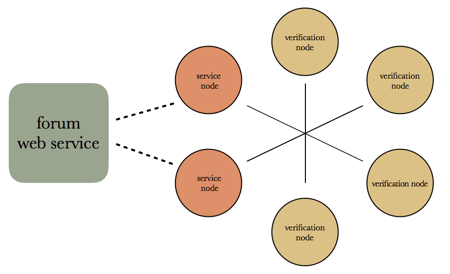
\includegraphics[width=0.8 \linewidth]{Network.png}
\caption{System Architecture}
\label{fig:system_architecture}
\end{figure}
The system architechture is shown in \ref{fig:system_architecture}. There are three major components
\begin{enumerate}
    \item ) Blockchain network verification node
    \item ) Blockchain network service node
    \item ) Web service node
\end{enumerate}
	
    Blockchain verification nodes and service nodes constitute the low level blockchain network. Verification nodes are used for verifying transactions and generating new blocks. Service nodes are designed to provide higher level service, such as block explorer, transaction search and system information search. Inside community system, service nodes are subjected to the community web service nodes, which provides necessary API for joining the community with the blockchain. Community web service nodes are user-orientated web services. It's responsible for new user registration and posting new threads. 

\section{UBFT Consensus Protocol}

\subsection{UBFT}
    UBFT stands for \emph{U network Byzantine Fault Tolerant} consensus algorithm, a novel consensus algorithm that combines the advantages of dPOS (Delegated Proof of Stake) algorithm and an improved Practical Byzantine Fault Tolerant (PBFT) algorithm\cite{pbft}. UBFT has two voting mechanisms built inside to keep the network secure from malicious attacks at all levels, while allowing all participants of the network to contribute to the security and performance of the system. 

\begin{figure}
\centering
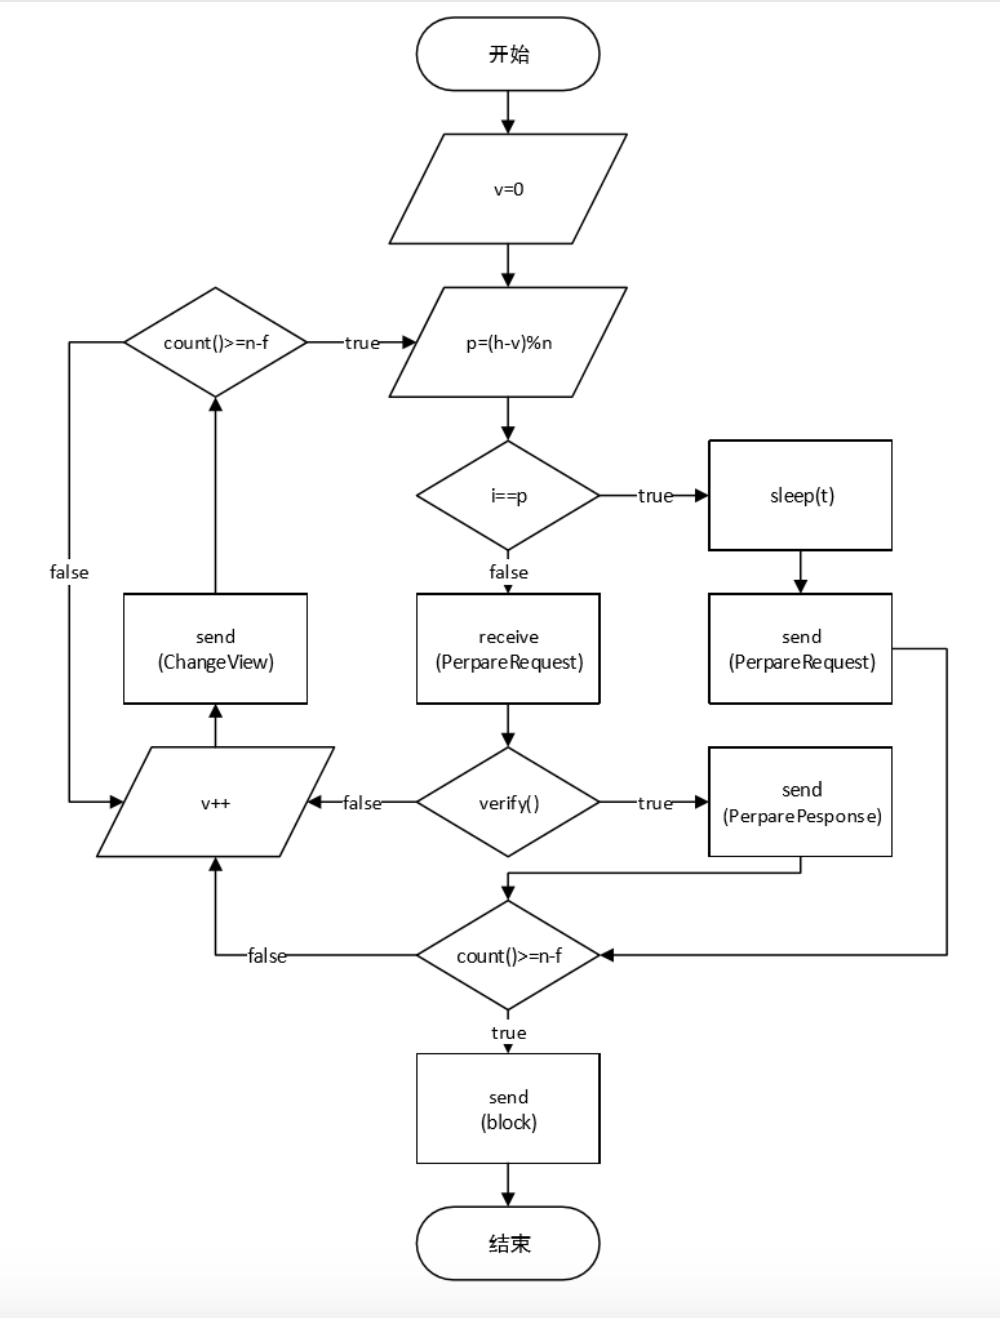
\includegraphics[width= 0.7 \linewidth]{consensus.png}
\caption{UBFT Flow Chart (source: A Byzantine Fault Tolerance Algorithm\cite{neo})}
\label{fig:ubft}
\end{figure}    
    
    The overall flow is shown in Figure \ref{fig:ubft}. This algorithm have a fault tolerant rate up to 1/3. Verification node is produced by voting. Only \emph{U Network} token stakeholders have the right to vote.  UBFT has following advantages:
\begin{enumerate}
    \item ) There will be no soft-fork. One confirmation is enough for a transaction. 
    \item ) No mining is needed, energy friendly.
    \item ) Adjustable block time. We expect the block time around 6 seconds. 
    \item ) Highly concurrent in comparison to traditional blockchain. 
    \item ) No delegates needed, while improving security and performance
\end{enumerate}



\subsection{Terms Used}
    \textit{Nodes} are blockchain participants that are connected to each other by peer-to-peer network, they can be running on different hardwares and operating systems and talk to each other by \textit{gossip protocol}, which is essentially a continuous broadcast protocol with signed content. Each \textit{node} maintain a full record of the blockchain history. \textit{SPV} clients are users with public address in the network, they can be running on a web browser, mobile phones, tablets, etc. \textit{SPV} clients don't maintain full records of the whole blockchain but rather those related to themselves.

    \textit{Verifiers} are \textit{nodes} that are elected by both other \textit{nodes} and interested \textit{SPV} clients to produce new blocks each \textit{round}. There could be multiple \textit{rounds} to produce a new block if consensus is not established in the first \textit{round}.

\subsection{Assumption of Protocol}
    It is of vital importance to keep a consensus protocol safe from malicious attack in a variety of forms, and yet a quantitative analysis on this matter is hard to define. To demonstrate and measure the safety of our protocol, we'll start by making a few assumptions.
\begin{enumerate}
    \item ) The network is partially synchronous, that is, there exists an unknown upper limit to the message delay between nodes.
    \item ) There are at most 1/3 of rogue nodes in the network.
    \item ) Nodes in the network are self-interested and there's no limit as to what malicious attackers can do.
\end{enumerate}
    We make these three assumptions so that we are able to further define our protocol. Specifically, we are not, and cannot define a consensus protocol that is Byzantium Fault-Tolerant in an asynchronous setting, as indicated by the FLP Impossibility result. While we assume there exists an upper limit to the maximum delay time in the network, the protocol does not use the knowledge of its value. Compared to alternative protocols such as DPOS, which assumes a synchronous network, our protocol is more applicable in a setting where nodes are running on different hardwares and there might be huge delays in between.

    We also assume that there has to be at least 2/3 honest nodes in the system, as it's the theoretical limit of any BFT algorithm.

    The third assumption implies that to establish a safe consensus protocol, a Nash equilibrium has to be established such that any deviation from the equilibrium leads to a net loss, which could be defined economically (such as Bitcoin) or through other means.

\subsection{Security of Protocol}
    UBFT is a derived version of PBFT algorithm, therefore as long as there are more than 2/3 honest nodes in the system, it is considered secure. While the ability to tolerate at most 1/3 failed nodes seems like a degradation from POW's 1/2 allowance (such as Bitcoin), one should be aware that UBFT, like other PBFT algorithms, is able to tolerate \textbf{any failure} instead of only crash. This improvement is crucial to our overall system design since U Network is designed to be able to host a wide spectrum of applications, which may result in different failure modes.
    In simple terms, the overall structure of the protocol could be stated as following.
\begin{enumerate}
    \item  UBFT produces block at roughly 6 seconds per block.
    \item  Every time a block is to be produced, a node in the system is elected to be the producer, and only the producer will be able \& required to generate a new block.
    \item  The producer is elected in a weighted round-robin fashion, with the weight being proportional to the amount of tokens deposited by each node and the votes they received from other nodes \& SPV.
    \item  The block produced by the producer might not be recognized by 2/3 majority of the system, in which case another producer will be elected, util a new block is produced.
    \item  The liveness of the system is guaranteed by the economic incentives for the nodes to correctly generate new blocks.
    \item  The election mechanism makes it possible for end users to contribute to the security of the system and thus restricted the power of full nodes.
\end{enumerate}

\subsection{Performance}

There are some popular metrics to evaluate the performance of a certain consensus protocol, to name a few, scalability, throughput and latency, etc.

In terms of scalability, it's more like a trade-off between scalability of adding new nodes and performance of transactions processing speed, as indicated by Vukolic M in one of his recent work \cite{bft_perf}. According to Vukolic, PoW protocol has an advantage of relatively higher node scalability since PoW used entirely distributed identity management, which means each node can download the full blockchain data and start participating the protocol. This is why PoW has been adopted by many public blockchain and so-called permission-less blockchain where anybody is allowed to participate. This feature enables PoW based blockchains to involve thousands of maintaining nodes, which guaranteed its decentralization. 

BFT and its derivatives, on the other hand, could only support a limited number of full nodes, practically less than 20. This is because the more nodes involved in the BFT consensus stage, the more messages need to be transferred and slower can reach consensus. Thus BFT-based consensus can offer a good performance in a small group of replicas, which brings criticism of its centralization.

\begin{figure}
\centering
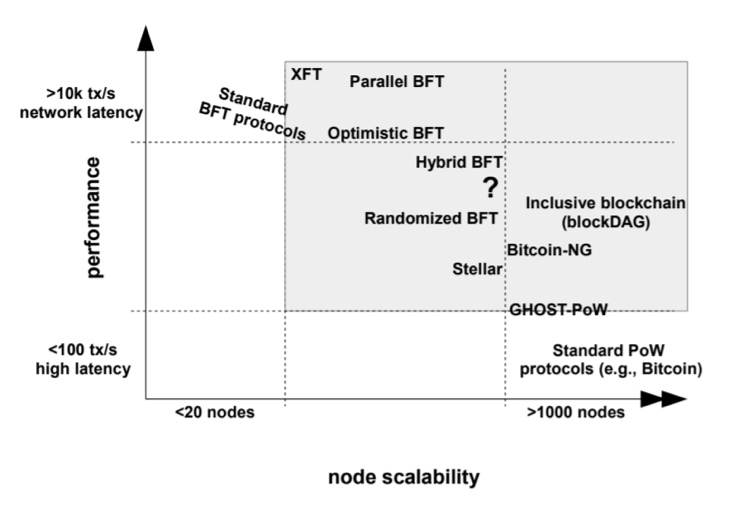
\includegraphics[width=  \linewidth]{bft_perf.png}
\caption{BFT Performance vs. Scalability}
\label{fig:bft_perf}
\end{figure}   

Based on the previous observation, UBFT tried to hit the sweet spot between the node scalability and performance. By carefully choosing the number of validation nodes, consensus can be reached in a considerable fast speed. At the same time, UBFT can also support thousands of transactions per second and matches the latency of network. In addition, the centralization could be avoided by adopting the delicate producer election process, which involve both the opinions from maintainers and platform users. By doing so, we tried to achieve an optimal balance between the scalability and the throughput performance, fit the demand of our applications and guarantee our decentralization philosophy.

%\subsection{Governance of Protocol}
%{\color{red} note: discuss how do we upgrade our consensus protocol in the future}


\section{Transaction Prococol}

%\subsection{Transaction Definition}
	In blockchain, transaction is defined as the change of ledger. It's a data structure compiled in binary that contains critical information like transaction type, transaction amount, sender address, and receiver address, time stamp, etc. All of these distinguish a transaction, and are used in both validating nodes and service nodes.  

    One major difference between \emph{U Network} blockchain and other blockchains is that we aim to make transaction types extensible, thus making it forward-compatible to applications. 
	
	Due to various types of user-generated-content products, we especially emphasize the extensibility of the system, as the growth of the decentralized \emph{U Network} could be booming one day. Therefore, by making transaction types extensible, we guaranteed the whole network is extensible without the need to change core internet protocol and consensus algorithm or storage structures.
	
	The system will support following major transaction types based on different scenario: 
	
	\begin{enumerate}
	\item )Asset register: used for coin mint
	\item )Asset publish: allocate users digital assets
    \item )Asset transfer: traditional UTXO transfer
    \item )Smart contract deploy: deploy compiled smart contract byte code to block chain
    \item )Smart contract message call: call deployed smart contract
    \item )Asset lock down: asset owner can lock the blockchain height
	\end{enumerate}
	
In order to defend against double-spent attack, all the pending transactions need to be confirmed sequentially in a deterministic way. Each validating node will have a pool of unconfirmed transactions. Given the efficiency of UBFT consensus algorithm, each verification node can verify up to 3000 transactions within 6 seconds of block time. To put it in another word, the blockchain can concurrently process 3000 transactions while keeping the transaction flow sequential. 



\section{Content Storage and Search}
\emph{U Network} internally leverages the IPFS (Inter Planetary File System \cite{ipfs}) for storing the content. IPFS is a distributed file system that seeks to connect all computing devices with the same system of files. In some ways, this is similar to the original aims of the Web, but IPFS is actually more similar to a single bittorrent swarm exchanging git objects. With IPFS, any content published in the IPFS network will be persistented forever, and accessed freely, easily and efficiently without being worried about the link expiration like HTTP. 

Meanwhile, on top of the IPFS storage, an abstract layer will be implemented in \emph{U Network} platform, to provide stable APIs to APP layers in service node, so it will easily plugin any other decentralized content storages, like Genero, into \emph{U Network} platform.

\subsection{Content Creation and Storage}
Once a piece of content is created in the \emph{U Network}, the content will be stored in IPFS and the hash to the content is returned, which will be used later for addressing. 

In the \emph{U Network}, the content address (the IPFS hash of the content) will be indexed in a smart contract. Every creation of a content will also result into a smart contract creation on the blockchain. The smart contract will have below states in the contract storage:
\begin{itemize}
\item The IPFS hash of the content.
\item The content creator's address. 
\item A list of upvoters' addresses, in sequential order.
\item A list of downvoters' addresses, in sequential order.
\item \emph{U Network} token balance. Voters' token balance used for voting will be transferred in and locked for delayed settlement. The settlement will be on demand performed per the settlement business rule, which is built-in in the smart contract.
\end{itemize}

\subsection{Content Search}

All the content created by \emph{U Network} will be grouped in an IPFS directory. There will also be an indexing file, mapping any content hash to the corresponding smart contract address. With this design, the browser will easily load the contents and their associated voters info. 

\subsection{Improvements}

A smart contract storing the content related info will be on the main blockchain initially. However, to achieve better scalability, \emph{U Foundation} plans to incorporate the state channel mechanism into \emph{U Network} platform at the next stage, like Aeternity. The content smart contract will then be created in the state channels. It will gain the below benefits using state channel:
\begin{itemize}
\item Activities on different content will be processed in parallel, and confirmed immediately.
\item It will keep the main blockchain efficient and clean.
\end{itemize}


\section{Token Incentive for Resources}

%Applications on blockchains consume three major types of resources:
%\begin{itemize}
%\item storage
%\item computation
%\item bandwidth
%\end{itemize}

\subsection{Storage Costs}
%{\color{red} note: Are we going to use IPFS for storage? If so, we need to discuss how.}
As a content blockchain platform, we need a significant amount of storage to store user-generated contents. These contents can take a large amount of space, especially for multi-media contents like vedios or pictures. These contents need to be stored in distributed network on participant nodes. Nodes who contribute storage spaces will be rewarded based on how much space they are providing.

\subsection{Bandwidth Costs}
The contents in \emph{U Network} will finally consumed by readers. To distribute contents to readers, network bandwidth will be consumed. To motivate paticipant nodes to relay contents to readers, we will account the bandwidth each relay nodes contribute and reward them with U Network tokens.

\subsection{Computation Costs}
All blockchain systems need nodes to verify transactions on top of it. \emph{U Network} will reward all nodes participating verification of a transaction when a transaction is successfully added to the public ledger, thus all nodes have the incentive to become a legit verification node. 


% chapter 3: U community Design
\chapter{\emph{U Community} - First Application in U Network Platform}
\section{Service Design}

As described in section 3.2, one of major components of \emph{U Network} is web service node. The cluster of service nodes will act as an aggregated service provider, which has inherent advantages due to the load-balancing and fault tolerant features of distributed systems. Each web service node implements a highly scalable and extensible protocol as the key component of forum services, which can process information with faster speed and improved stability. 

The forum data will be stored across the web service nodes, which guarantees the availability and consistency of user data due to redundant duplicates. In this way, each time users make an interaction with the \emph{U Network}, they actually make a \emph{https} request to one of the available web service nodes. For efficiency consideration, each request may include one or more on-chain transaction requests that interact with the \emph{U Network} blockchain. 
\subsection{Topic Mechanism}
\emph{U Community} content is organized by topic mechanism. Similar to XUE QIU\cite{xueqiu}, each digital asset will formulated as a ``topic'', which contains both user generated contents and platform generated contents belonging to the same type of asset. Here, the platform generated contents include general information, news and announcements in \emph{U Community}. As such, users can browse both the platform information and other user generated contents with the similar topic.  
\subsection{Publish and Subscribe}
\emph{U Community} content distribution is based on the publish and subscribe model. Contents creator can publish their articles or any other digital assets in the community, while audience can subscribe creators or topics and receive new updates. In the mean time, users can cancel their subscription anytime when the contents or topic becomes unattractive to them. 
\subsection{Content Ranking}
%{\color{red} note: need to discuss how to rank the order of the vote}
%{\color{blue} could move the vote ranking explanation from 3.4 to here}

\emph{U Community} constructs a content-value prediction market to promote quality contents to more audience. As the critical component, it is very important to rank the stream of contents and their votes so that to determine their sequential orders. The ranking algorithm can be represented by the formula below:
\begin{center}
$f(t_s,y,z) = \log_{C} z + \frac{y * t_s}{45000}$
\end{center}
\  $t_s$ denotes the lifetime of the post which is the time period since content is created:
\begin{center}
    $t_s = T_{posted} - T_{created}$
\end{center}
$y$ is the indicator function and \ $y \in \{-1,0,1\}$
$$y =\left\{
\begin{array}{rcl}
1       &      & {if \quad x > 0}\\
0     &      & {if \quad x = 0}\\
-1     &      & {if \quad x < 0}
\end{array} \right. $$
\ $x$ is the count difference of up-votes and down-votes
\begin{center}
        $x = U - D$
\end{center}
\  $U$ is the weighted sum of upvotes, while\ $D$ is the weighted sum of downvotes. Specifically, $w_{U}^{i}$ is the weight of voter for $i$-th up-vote, while $w_{D}^{i}$ is the weight of voter for $i$-th down-vote.
\begin{center}
$U = \sum_{i=1}^{N} w_{U}^{i}$
\end{center}
\begin{center}
$D = \sum_{i=1}^{N} w_{D}^{i}$
\end{center}

The weight of each vote is calculated by taking the logarithm of total up-votes prior to itself, and adding with the deposited \emph{U Network} tokens. \emph{U Community}  users can purchase \emph{U Network} tokens and enjoy more privilege by locking up their tokens into deposit. Note that only deposited tokens can empower their owner with the extra voting power. \par

By reducing the liquidity of \emph{U Network} tokens, the stakeholders' interests can better align with that of the community. In this way, users become more cautious in their voting because their voting decisions have more direct connection with their own interest. This mechanism can better eliminate arbitrary votes which jeopardize the fairness and effectiveness of the platform. Therefore, \emph{U Network} token holders are more likely to make prudent judgments for the community and should be given more voting power.

Meanwhile, the logarithm operation prevents major stakeholders from owning unconstrained dictating power.
All of these combined with the number of upvotes can quantify the user's expertise as: 
\begin{center}
        $w_{U, D}^{i}$ = $max(0, log_M r) + max (0, log_N t)$
\end{center}
$M$ and \ $N$ are two constants, subjects to changes up-on agreement of the community;
\ $z$ simply choose the larger one between $|x|$ and 1.
$$z =\left\{
\begin{array}{rcl}
|x|       &      & {if \quad |x| \geq 1}\\
1     &      & {if \quad |x| < 1}\\
\end{array} \right. $$

$C$ denotes cool-down constant. To make it clear, $C$ is the base of logarithm inside $\log_{C}$ $z$. As an example, when $C = 10$ it means $\log_{C} z = 1$ when $z = 10$. Similarly,  $\log_{C} z = 2$ when $z = 100$. Obviously, the first ten voters share a similar weight with the following 90 voters, (and even 100th to 900th voters). It means that for a popular post, the weight is decreasing as the rank of voters is increasing. In other words, the up-vote has less impact when $C$ becomes larger.

The number ``45000'' in the denominator has unit of second, which equals to 12.5 hours. It means that posts which was published one day before need to have 100X more votes to sustain its original ranking at current time. As such, \emph{U Network} tends to promote latest new contents but still gives high rank to very popular contents.  

As an important ranking factor, the sequential order of votes is critical to determine both posts ranks and participants rewards. We need a fair and trustworthy judgment using ``smart contract''. In details, each vote can be considered as a micro-payment, which is time-stamped, and paid to a smart-contract address. Each time stamp is an unsigned 64 bit integer, and the value is assigned by the validating node. The smart contract can access the time stamp to assign the order-based \emph{U Network} token rewards. To prevent the \emph{Time Travel} attack, each verification node will only accept transactions whose time stamps are in the valid range. Therefore, no malicious user can modify the time stamp of the vote to cut in the middle of voting sequence and receive undeserved rewards.  

\section{Community Role Design}
\emph{U Community} is composed of regular users, content creators, content explorers, and community moderators. 
\subsection{Regular Users}
Regular users can transform into different roles. First, they receive points by completing a given set of micro tasks. In addition, they can become content creators by posting new contents. Also, they can behave as content explorer by discovering and up-voting topics. Moreover, they can be chosen as community moderator.  
\subsection{Content Creators}
Content creators are the most important contributors in the development of \emph{U community}. They will receive \emph{U Network} tokens as rewards according to the quality of generated contents. 
\subsection{Content Explorers}
Content Explorers are users who up-vote to discover and promote high-quality contents for the community. If their promoted contents are appreciated by more users, they can receive \emph{U Network} tokens as rewards. 
\subsection{Community Moderators}
Community moderators are selected periodically from regular users. The probability of a user being selected is proportional to the \emph{U Network} tokens they are holding. As an incentive, they are rewarded with \emph{U Network} tokens for serving as the moderator.

The function of community moderators is to ensure the smooth operation of \emph{U Community} without turbulence. In addition, moderators have privilege in determining future movement of the community. 

One of the most important privilege of moderator is the ability to delete improper topics. To restrict moderator and prevent abuse of such power, authors of deleted contents can appeal which require a significant amount of \emph{U Network} tokens deposit. In the meantime, other  audience in the community can vote to express their opinions in the appeal process. Each vote would cost small amount of \emph{U Network} tokens to prevent spam voting. After appeal period finishes, the supporters of the deletion is dominant (e.g., more than 50\% of total participants), the appeal initiator would lose the deposit and the users who supported the appeal would also lose their \emph{U Network} tokens spent in the voting process. Vice-versa. 

The formula to assign rewards for the majority voter is calculated as follows. 
\begin{center}
    $${p}=({N}*{c} - {F})/{N_w}$$
\end{center}
$p$ is the reward for each users winning the appeal. $N$ is the total number of the users voting for the appeal. $c$ is the cost of casting a vote. $F$ is the processing fee goes to the platform. $N_w$ is the number of majority. This formula ensures each voter will have to use her best judgment to analyze the situation to gain rewards in the end, therefore, preventing trolls casting arbitrary votes. 


After the first appeal voting period there is a cool-down period, in which if either the appeal initiator or the community moderator is unsatisfied with the result. They can start a second round of appeal. The extra appeal would require exponentially more deposit than the previous appeal. If the second appeal result is different from the previous one, the reward allocation for the previous one is canceled and the final rewards are allocated based on the second appeal result.

This process is repeated until both parties reach an agreement or either one party choose to exit the appeal process. 
Community moderators will automatically assign partial of received \emph{U Network} tokens distribution to users supporting them. However, if the appeal result revokes the original deletion, those \emph{U Network} tokens would be rewarded to users who disapproved of the deletion.  
\section{Token Incentive Design}
\emph{U Network} tokens represents the right to use \emph{U Community} and its related applications. It's the connection between rewards and contents and, similarly, the connection between users.

\emph{U Network} tokens is the value carrier of the \emph{U Community}. The larger users \emph{U Community} attracts, the more quality content is produced. \emph{U Network} tokens, with limited total supply, would benefit all the \emph{U Network} tokens holders when more high-quality contents are created in the community and the demand of tokens increases.  From this point of view, \emph{U Network} users are not only customers of the platform, but also beneficiaries if the community thrives in the long term. 
	
\subsection{Incentives for Content Creators, Explorers, and Moderators} 
To motivate participants in \emph{U Community} to make their contributions, both high-quality content creator and content explorer will receive \emph{U Network} tokens as rewards.

Each user can either ``up-vote'' or ``down-vote'' a piece of contents with a small amount of token as the cost. Contents being down-voted would be degraded and eventually disappear in the community with a lot of down-votes. Thus trolling content would not be spread across the network. 

There are two major sources of \emph{U Network} tokens rewards for content creators and content explorers. One is purchase of \emph{U Network} tokens in the exchange, the other source is to convert reward points received from completion of micro tasks into \emph{U Network} tokens. Those points are gradually released from the system, called ``content-reward pool''. There is a limit on the number of points that can be released daily, and the ``content-reward pool'' will shrink to be empty eventually. This policy is set to attract users to receive points by discovering high-quality contents at early stage. 

Note that the platform will charge 5\% of token distribution for the reward assigned to content creators and explorers, which ensures the stability and sustainability of the \emph{U Community} economy model.

%\subsection{Socialized Investment, Smart-contract based Co-investing}
%Investors can choose to upload trading strategies and order history to \emph{U Network}  to make future decisions in an organized fashion. Also,seasoned investors can share their trading strategies with the whole community, and provide relevant technical or fundamental analysis. Other users can pay to view such content, and become an co-investor of such strategies. With the help of smart contracts, \emph{U Community} provides a decentralized, reliable way for users to control their own assets, and automatically, completely imitates/clone professional investor's strategy. If the following user made profit by doing so, the smart contract will carry part of the profit to the author of the original strategy. 
%In the future, users can use \emph{U Network} tokens to purchase \emph{U Community} platform investment advice from trusted third party applications. 
%\subsection{Survey, Voting, Prediction Market}
%\emph{U Community} will provide a way for user to receive token rewards by conducting survey, which greatly increase the completion rate of survey in the community. \emph{U Community} will release products with built-in prediction market and support native prediction markets that are extensible, efficient and accurate.
%\subsection{Incentive for Advertisement}
%High-quality contents deserves to be promoted to more audience.  \emph{U Community} can help promote information to target audience with specific characteristics. While spreading fake or irreverent content will be punished.  
%Off site collaborators will also be able to publish advertisements inside \emph{U Community}. However, the content will be strictly reviewed by the community moderators. All the revenue will contribute to the content-reward pool. 

%\subsection{Incentive Gift}
%Sending \emph{U Network} tokens as a reward is an efficient way of interaction between community celebrities and fans. It's good community culture to pay reward to those who you have been receiving help from. Posts receiving higher rewards will have a higher exposure in the community. Users can pay \emph{U Network} tokens to unlock extra features like medal and skins. 5\% of the reward will go to 'content-reward pool'. The rest will be received by the beneficiaries. 

\subsection{Incentive for Knowledge Sharing}

Users can pay \emph{U Network} tokens to request private interactions with creators of high-quality contents, and receive personalized comments. In this way, creators receive token incentive and are motivated to share more knowledge information to their audience in three types of interaction: paid Subscription, paid Q\&A, pay to message. 
Paid subscription provides a way for creators to make monetary profit with their knowledge and influence. After receiving a given amount of up-votes, content creators can setup a private group or private channel to provide more insightful information to audience who are willing to pay \emph{U Network} tokens as subscription fee. 
	
Users can also choose a more active interactive approach. After paying a certain amount of \emph{U Network} tokens, users can ask specific questions to content creators. The answer can be set visible to the public or in private, and other audience need to pay to ``peek'' the conversation.
						
The third approach is messaging between creators and audience. To filter unsolicited messages, creators can set minimal token cost that has to be paid in order to send a private message. Audience can become more cautious to send meaningful messages in the same time.


% chapter 5: RoadMap
\chapter{Future Direction and Roadmap}

\section{Future U Network Evolution}
As the exponential growth of information continues in the next few years, we believe \emph{U Network} is the best solution to the problems of traditional user-generated-contents communities. With the blockchain technology and economic incentive model, \emph{U Network} constructs a content-valuation prediction market. It provides reasonable incentives to valuable-content creators, and motivates the regular user audience to explore and promote high-quality contents. Therefore, high-quality contents can easily stand out and all contributors receive their monetized rewards in the \emph{U Network}.

Moreover,  \emph{U Network} construct an ``user-generated-content public blockchain'', which serves as the framework and platform of future content-oriented communities and applications. In particular,  \emph{U Community} will be the first application using  \emph{U Network} platform which focuses on the content information of digital assets.

In the long term,  \emph{U Network}  will fully utilize the distributed storage protocol to further improve the decentralized platform infrastructure, which emphasize on data integrity and user privacy.  In addition, innovative consensus algorithm will be implemented to further expedite the transaction speed and enhance the reliability of transactions. Moreover, performance optimization will be proposed for decentralized search algorithm, therefore, making it more efficient to identify up-voters for valuable contents. 

\section{Future Application Use Case}
In the era of information explosion, \emph{U Network} opens the door to a huge market for user-generated contents. It is an revolutionary trend to empower creators, distributors and explorer of high-quality contents, who are the driving force of future valuable-content communities. Therefore, all existing communities and applications can be revolutionized using \emph{U Network} in different industries. 

 \subsection{Communities for Valuable Digital Literature}
For communities with constantly updated series of literature contents, it's imperative to rate the published content and motivate the author to maintain the quality in the following release. By introducing \emph{U Network} rating and rewarding system, top-selling authors can receive a long-term incentive and reasonable returns.  


 \subsection{ Communities for Digital Asset}
More people include digital assets, such as crypto-currency\cite{bitcoin,eth,eth2}, into their asset portfolio in the past decade. Those people need a community to gather reliable information, exchange opinions and learn from professionals. However, existing communities are notorious for fake information and fraudulence. Users find it very challenging to identify reliable and valuable information. As such, \emph{U Network} provides the best solution as high-quality contents can be discovered easily and promoted to more audience.  

 \subsection{Communities for Knowledge Sharing}
There are some issues with existing knowledge-sharing communities like Quora and Zhihu: authors have no direct and reliable approach to convert their knowledge into monetized rewards. In this scenario, \emph{U Network} can reward creators of valuable contents based on its rating and reward incentive mechanism. 

 \subsection{Communities for Social Media}
Existing social media communities such as blog and forum are important for regular Internet users to broadcast their own contents. With \emph{U Network} framework, these communities can construct their own rating and reward mechanism. As such, contributors of valuable contents in these existing communities can receive profit rewards. 

 \subsection{Communities for Intelligent Property}
Current society respect the original ownership of intelligent property, such as music, video, and articles. Nearly all these contents need content rating mechanism to discover and recommend high-quality ones. These communities can easily integrate \emph{U Network} framework and setup their own rating and reward system for specific intelligent property. 


\section{Roadmap}

	\begin{itemize}

	\item Jun 2015 to now, \emph{U  Network} team has been focusing on technology contents which had attracted more than 4 million active users. 
	\item Aug 2017, partnered with Huobi, we presented ``From 0 to 1, learn blockchain technology in a comprehensive way''. Over 10,000 paid students have completed the program. 
	\item Sept 2017, we launched ``Smart Contract Development'' education program. More than 180 blockchain developers had graduated from this program.    
	\item Jan 2018, we had hold ``Blockchain Connect'' China-US blockchain summit in San Francisco.
	\item Aug 2018, \emph{U  Network} Testnet release
	\item Nov 2018, \emph{U  Network} Mainnet release
	\item Dec 2018, \emph{U Community}  Alpha version release. 
	\item Feb 2019, \emph{U  Network} optimized Mainnet release
	\item May 2019, \emph{U Community} Beta version release, supports co-investing functionality
	\item Aug 2019, Completing \emph{U  Network} Mainnet and developer tool kits,
	\item Dec 2019, Build \emph{U  Network} ecosystem, import \emph{U  Network} into exisiting UGC platforms. 
\end{itemize}

% chapter 6: conclusion
\chapter{Conclusion}

We have introduced \emph{U network}, which is a revolutionary content-value based prediction market platform and a content-incentive community powered by blockchain technology. In this platform the valuable contents are encouraged to be created and discovered by all participants with the rewards of monetized tokens.  

The long-term goal of \emph{U Network} is to build a decentralized user-generated-content community, where high-quality contents can be created, discovered and promoted to more audience in an efficient approach. To motivate all participants, regular users needs to pay \emph{U Network} token as cost in order to access high-quality contents, while other contributors will receive \emph{U Network} tokens as an incentive. Both content creator and explorer can be rewarded for their different contributions. As such, the platform brings plenty of value to all participants. 

In particular, \emph{U} Community will be the first digital asset platform powered by \emph{U network} blockchain technology. \emph{U Network} team believes that more decentralized user-generated-content applications will be deployed on the \emph{U Network} public blockchain in the near future. \emph{U Network} will bring revolutionary changes to each different industry.






\appendix
\chapter{To-Do List}

The \emph{U  Network} is an open-source project that can be found at ``https://github.com/U-Network/UNetwork''. At the early stage of development, there are many tasks need to be finished. Partial work on the list is following:


\begin{enumerate}

\item {\bf Revision of Document}: 
\begin{enumerate}
\item Revise README document and composite a short version. It should clearly explain the fundamental blockchain system of  \emph{U  Network}, provide summary of features, and point out future directions. 
\item Remove docus/specification directory.
\item Add more documents regarding testing and deployment of  \emph{U  Network}.
\end{enumerate}

        

\item {\bf Coding Style Convention}: 
\begin{enumerate}
\item Current coding style is inconsistent. It is advisable to modify the entire code repository.
\item Suggested Golang coding standard: 

\textit{https://github.com/golang/go/wiki/CodeReviewComments}
\end{enumerate}

\item {\bf Redundant Code Removal}:
\begin{enumerate}
\item remove directories: cli/LevelDBQuery, cli/consensus, consensus/sbft, net/rpt\_test
\item remove files: account/account\_test.go, consensus/policy.go, consensus/policyLevel.go, core/transaction/txAttribute\_test.go
\end{enumerate}

\item {\bf Continuous Integration}:
\begin{enumerate}
\item Use Travis CI to automatically compile and build after each check-in delivery.
\end{enumerate}


\item {\bf Bug Fix and Improvement}:
\begin{enumerate}
\item  move the hash generation of transaction into core/transaction/TransactionBuilder.go
\item  enforce consistent address format of registered asset, such as prefix.
\item modify the redundant interface of RPC. 
\end{enumerate}


% external end
\end{enumerate}


\clearpage


%\begin{thebibliography}{9}
\bibitem{prediction} 
Justin Wolfers and Eric Zitzewitz and Justin Wolfers and Eric Zitzewitz,
``Prediction Markets''. 
\textit{J. Economic Perspectives}, 2004. Page(s): 107--126

\bibitem{steem} 
Steem, 
``Steem an incentivized, blockchain-based, public content platform'', 2017
\\\texttt{https://steem.io/SteemWhitePaper.pdf}


\bibitem{primas} 
Primas, 
``Primas next generation ecosystem for valuable content'', 2017
\\\texttt{https://primas.io/pdf/primas-1.3.1-en.pdf}

\bibitem{pbft} 
Castro, Miguel and Liskov, Barbara. 
``Practical Byzantine Fault Tolerance''. 
\textit{Proceedings of the Third Symposium on Operating Systems Design and Implementation}, Berkeley, CA, USA, 1999. Page(s): 173--186

\bibitem{efficient} 
J. S. Jordan. 
``On the efficient markets hypothesis''. 
\textit{Econometrica}, 1983. Page(s): 1325--1343


\bibitem{bitcoin} 
Satoshi Nakamoto, 
``Bitcoin: A peer-to-peer electronic cash system''. 2008
\\\texttt{http://bitcoin.org/bitcoin.pdf} 

\bibitem{eth} 
Vitalik Buterin, 
``A next-generation smart contract and decentralized application platform''. 2014
\\\texttt{https://github.com/ethereum/wiki/wiki/White-Paper} 

\bibitem{eth2} 
Gavin Wood, 
``Ethereum: a secure decentralised generalised transaction ledger''. 
\\\texttt{http://gavwood.com/paper.pdf} 

\bibitem{ipfs} 
Juan Benet, 
``IPFS - Content Addressed, Versioned, P2P File System''. 2014
\\\texttt{https://arxiv.org/abs/1407.3561} 

\end{thebibliography}
 


\bibliographystyle{unsrt}
\bibliography{reference}

%\printbibliography

\end{document}

